% !TEX root = ../ausarbeitung.tex
%Unter Evaluation der Result Teil mit "nackten Zahlen" als Boxplot + Textuell %Mittelwert und Standardabweichung. Wenn möglich noch ein statistischen Test %zwischen den einzelnen Kategorien.
\chapter{Results} %TODO Ref
In diesem Kapitel werden die Ergebnisse des Nutzertests präsentiert. Die Darstellung erfolgt nach den Kategorien, die durch den GEQ definiert wurden. Anhand von Boxplots werden die Ergebnisse der jeweiligen Kategorie von der ThirdPerson Ansicht und der TopDown Ansicht gegenüber gestellt.
\section{Challenge}
\begin{figure}[h!tb]
	\centering
	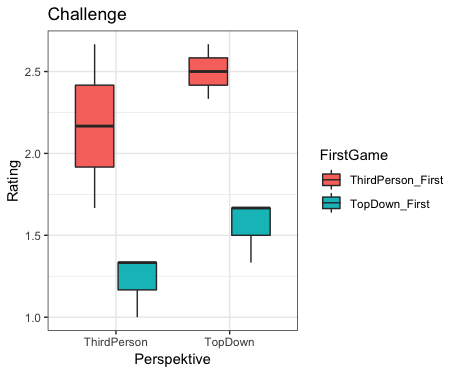
\includegraphics[width=0.65\textwidth]{challengePlot}
	\caption{Boxplot der Kategorie Challenge\label{fig:farbskala}}
\end{figure}
Der Durchschnitt in der Challenge Kategorie beträgt für TopDown zuerst $1.8\overline{8}$
\section{Competence}
\begin{figure}[h!tb]
	\centering
	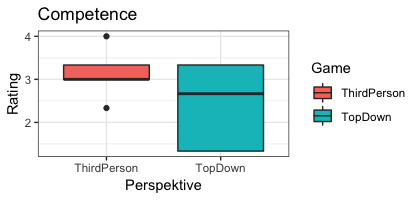
\includegraphics[width=0.65\textwidth]{competencePlot}
	\caption{Boxplot der Kategorie Competence\label{fig:farbskala}}
\end{figure}

\section{Flow}
\begin{figure}[h!tb]
	\centering
	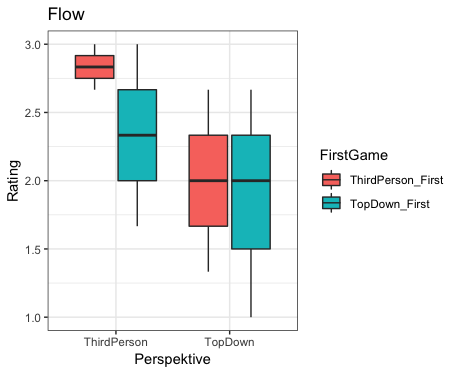
\includegraphics[width=0.65\textwidth]{flowPlot}
	\caption{Boxplot der Kategorie Flow\label{fig:farbskala}}
\end{figure}

\section{Immersion}
\begin{figure}[h!tb]
	\centering
	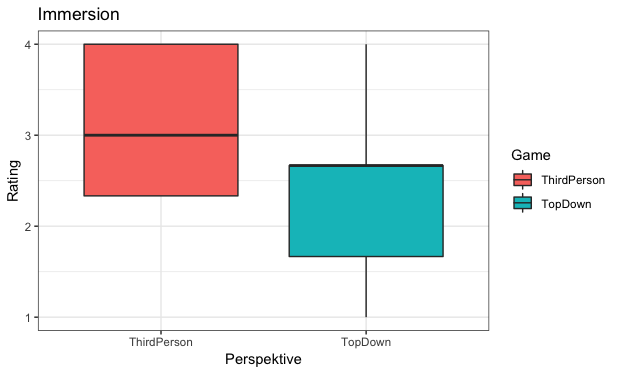
\includegraphics[width=0.65\textwidth]{immersionPlot}
	\caption{Boxplot der Kategorie Immersion\label{fig:farbskala}}
\end{figure}

\section{Negative Effect}
\begin{figure}[h!tb]
	\centering
	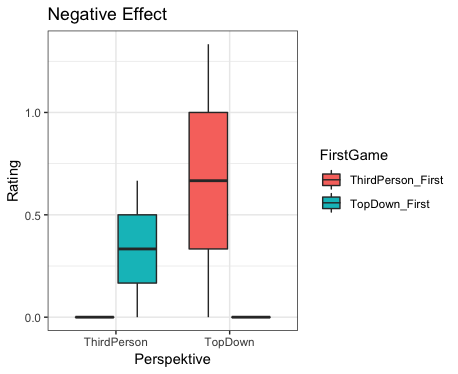
\includegraphics[width=0.65\textwidth]{negEffPlot}
	\caption{Boxplot der Kategorie Negative Effect\label{fig:farbskala}}
\end{figure}

\section{Positive Effect}
\begin{figure}[htb]
	\centering
	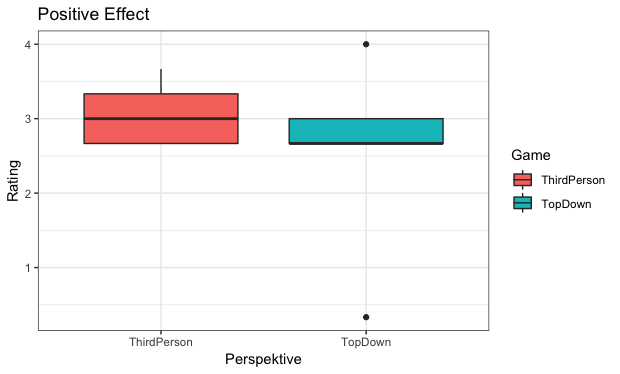
\includegraphics[width=0.65\textwidth]{posEffPlot}
	\caption{Boxplot der Kategorie Positive Effect\label{fig:farbskala}}
\end{figure}

\section{Tension}
\begin{figure}[htb]
	\centering
	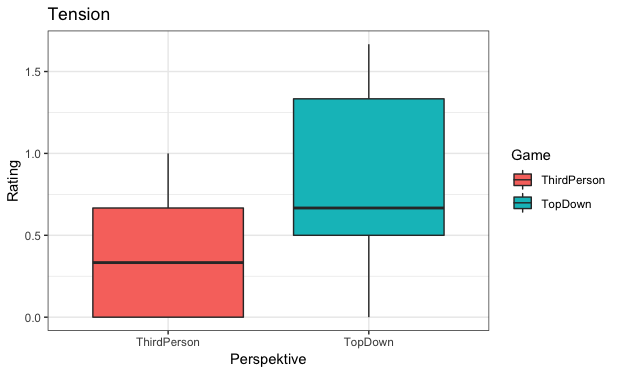
\includegraphics[width=0.65\textwidth]{tensionPlot}
	\caption{Boxplot der Kategorie Tension\label{fig:farbskala}}
\end{figure}

\hfil\rule{0.4\textwidth}{0.4pt}